\documentclass{article}
\usepackage{amsmath}
\usepackage{amssymb}
\usepackage{graphicx}
\usepackage{hyperref}
\usepackage[version=4]{mhchem}

\title{Problem 13}
\date{}

\begin{document}
\maketitle

\section*{Problem}
As shown in the figure, in trapezoid \(A B C D, \angle A+\angle B=90^{\circ}\). Find \(E F\) if \(A B=a, C D=b . E\) is the midpoint of \(A B\) and \(F\) is the midpoint of \(D C\).\\
(A) \(\frac{1}{2}(a+b)\).\\
(B) \(\frac{1}{2}(a-b)\).\\
(C) \(\sqrt{a^{2}+b^{2}}\).\\
(D) \(\sqrt{a^{2}-b^{2}}\).\\
\centering
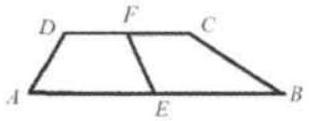
\includegraphics[width=\textwidth]{images/128(4).jpg}

\section*{Solution}
Solution not available.

\end{document}
